\qquad A análise de complexidade do Merge Sort, considerando as
diferentes situações de entrada (crescente, decrescente e randômica),
foi realizada manuscrita, com a devida justificativa, contando o número
de execuções de cada linha da função de intercalação (associando uma
constante de custo $c_i$ a cada linha), escrevendo a recorrência da
função recursiva e resolvendo-a, conforme exigido pelo enunciado do
trabalho.

\begin{figure}[htbp]
    \centering
    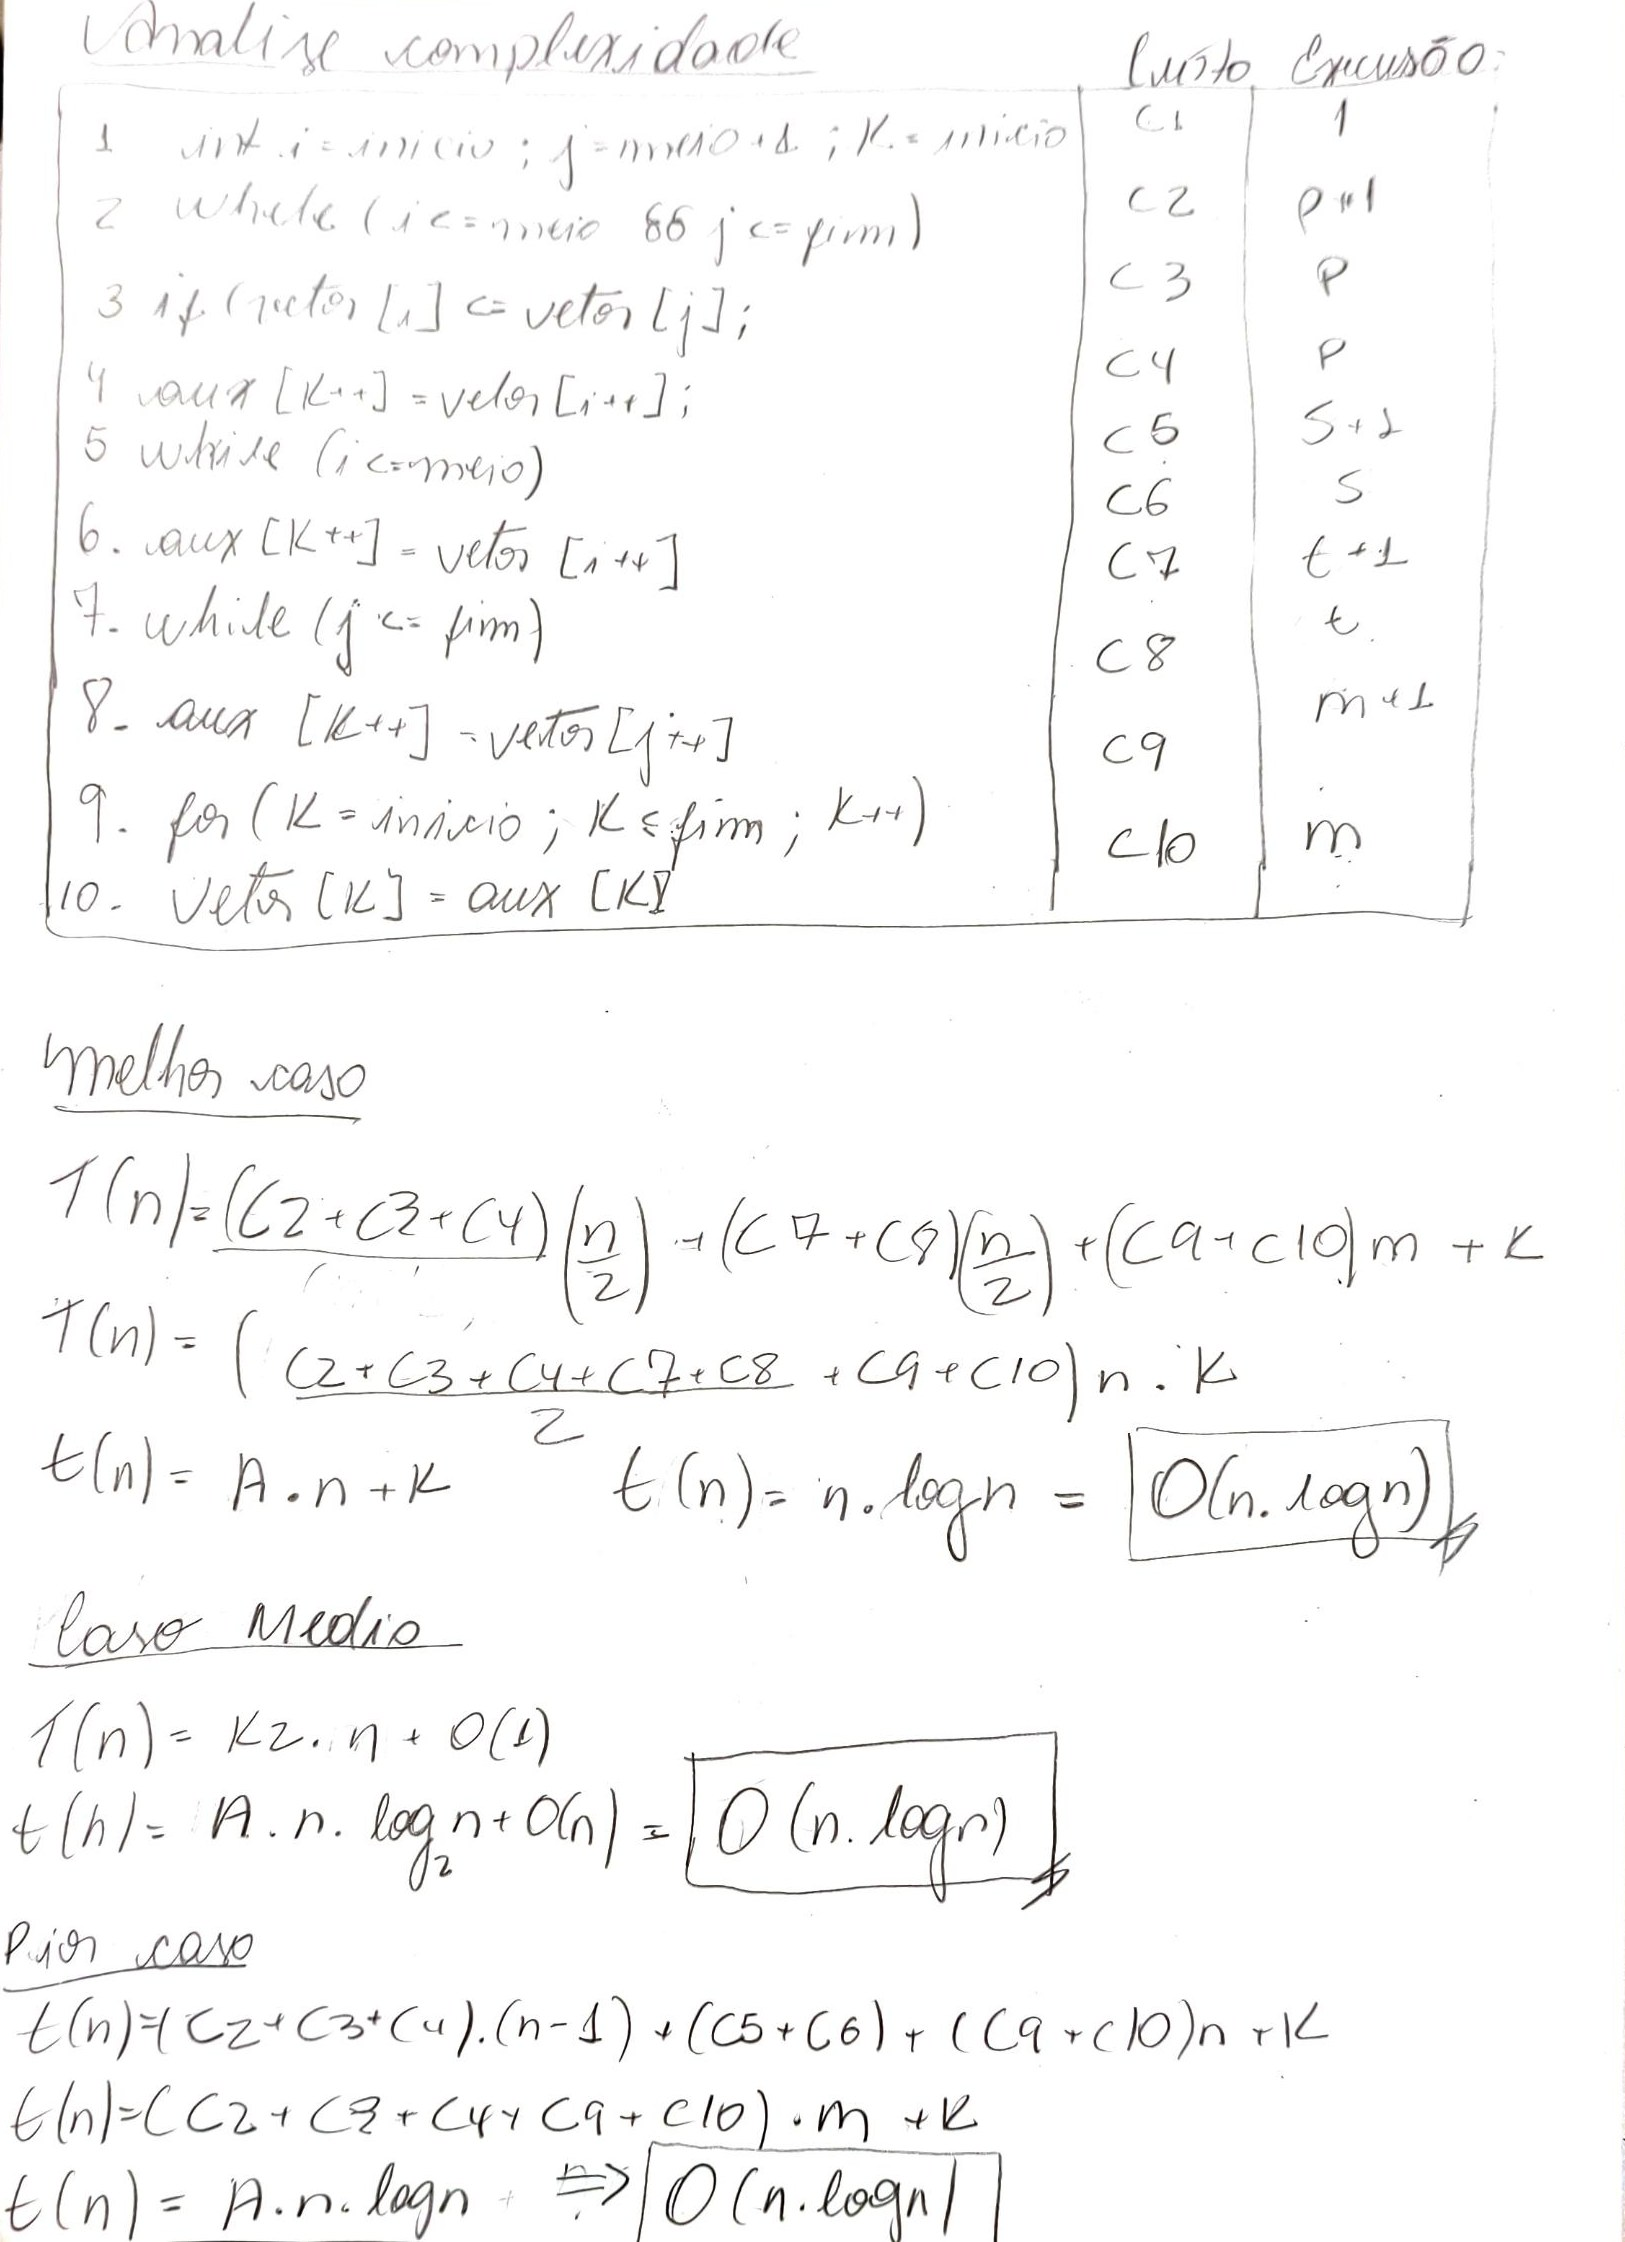
\includegraphics[width=14cm]{Imagens/Merge Sort/analise_complexidade.png}
    \caption{Análise de complexidade manuscrita do algoritmo Merge Sort}
    \label{fig:analise_complexidade_merge}
\end{figure}

\qquad Em resumo, a análise manuscrita chega às seguintes conclusões.
\textbf{Intercalação:} para intercalar um trecho de $m$ elementos, seja
$p$ o número de iterações do primeiro laço (que é também o número de
comparações) e sejam $s$ e $t$ os elementos que restam, respectivamente,
na metade esquerda e na direita quando a outra se esgota. Como cada
elemento é copiado exatamente uma vez para o vetor auxiliar,
$p + s + t = m$. Somando as execuções de cada linha de
\texttt{Intercalar}, obtém-se
$T_I(m) = (c_2+c_3+c_4)\,p + (c_5+c_6)\,s + (c_7+c_8)\,t + (c_9+c_{10})\,m + K$,
com $K$ constante. Como todos os coeficientes são positivos e
$p + s + t = m$, resulta $T_I(m) = \Theta(m)$ em qualquer situação: o
que varia de uma entrada para outra é apenas como os $m$ elementos se
dividem entre $p$, $s$ e $t$.

\qquad \textbf{Recorrência:} \texttt{MergeSortRecursivo} faz duas chamadas
sobre metades do vetor e uma intercalação, ou seja,
$T(n) = 2\,T(n/2) + T_I(n) + c = 2\,T(n/2) + \Theta(n)$, com
$T(1) = \Theta(1)$. Como o vetor pode ser dividido ao meio $\log_2 n$
vezes até restarem trechos de um único elemento, a árvore de recursão
tem cerca de $\log_2 n + 1$ níveis e, em cada nível, as intercalações
percorrem, no total, os $n$ elementos do vetor, a um custo
$\Theta(n)$ por nível. O custo total é, portanto, $\Theta(n \log n)$ ---
resultado que também decorre do caso 2 do Teorema Mestre
(CORMEN et al., 2009), com $a = 2$, $b = 2$ e $f(n) = \Theta(n)$.

\qquad \textbf{Melhor caso (entrada crescente ou decrescente):} em cada
intercalação, todos os elementos de uma das metades são menores que os
da outra; assim, o primeiro laço termina após cerca de $m/2$ comparações
e o restante da outra metade é copiado diretamente. O custo
$T_I(m)$ continua linear, e a recorrência não muda, de modo que
$T(n) = \Theta(n \log n)$, com cerca de $\tfrac{n}{2}\log_2 n$
comparações no total.

\qquad \textbf{Pior caso:} ocorre quando os elementos das duas metades se
alternam em todas as intercalações; o primeiro laço só termina após
$p = m - 1$ comparações, totalizando $n \log_2 n - n + 1$ comparações
(para $n$ potência de 2). Ainda assim, $T(n) = \Theta(n \log n)$: apenas a
constante é maior. Nenhuma das três entradas testadas é exatamente esse
pior caso.

\qquad \textbf{Caso médio (entrada randômica):} as duas metades se
entrelaçam de forma aleatória e, quando uma delas se esgota, restam em
média apenas poucos elementos da outra; logo, $p$ fica próximo de $m - 1$
e o número de comparações fica próximo do limite do pior caso, com
$T(n) = \Theta(n \log n)$.

\qquad Diferentemente do Insertion e do Bubble Sort,
\textbf{melhor, médio e pior caso têm, portanto, a mesma complexidade},
$\Theta(n \log n)$, pois a divisão e a intercalação são executadas por
completo qualquer que seja a ordem dos dados. O número de comparações
fica sempre entre $\tfrac{1}{2} n \log_2 n$ e $n \log_2 n$
(SEDGEWICK; WAYNE, 2011), e o número de cópias de elementos é o mesmo em
todos os casos, cerca de $2n\log_2 n$.

\qquad Para conferir essa previsão, foi executada uma versão do algoritmo
instrumentada para contar as operações (usada apenas para esta
verificação, fora do código entregue) sobre 1.000.000 de elementos:
foram contadas 10.066.432 comparações para a entrada crescente,
9.884.992 para a decrescente e 18.673.990 para a randômica, valores
compatíveis com os limites teóricos de, respectivamente, cerca de
9.965.784 ($\tfrac{n}{2}\log_2 n$) e 18.931.570 ($n \log_2 n - n + 1$) --- as
pequenas diferenças decorrem de 1.000.000 não ser uma potência de 2.
O número de cópias foi de 39.902.848 nos três casos, ou seja, cerca de
$2n\log_2 n$, independentemente da ordem da entrada.

\qquad Em contrapartida, o algoritmo exige memória adicional proporcional a
$n$ (o vetor auxiliar), enquanto Insertion, Selection, Bubble e Shell
Sort ordenam no próprio vetor, com memória adicional constante. Os
resultados experimentais apresentados na próxima seção deste capítulo
são compatíveis com essa análise: os tempos das três entradas cresceram
aproximadamente na proporção $n \log n$, sem a explosão quadrática
observada nos três primeiros algoritmos.
